189. \begin{figure}[ht!]
\center{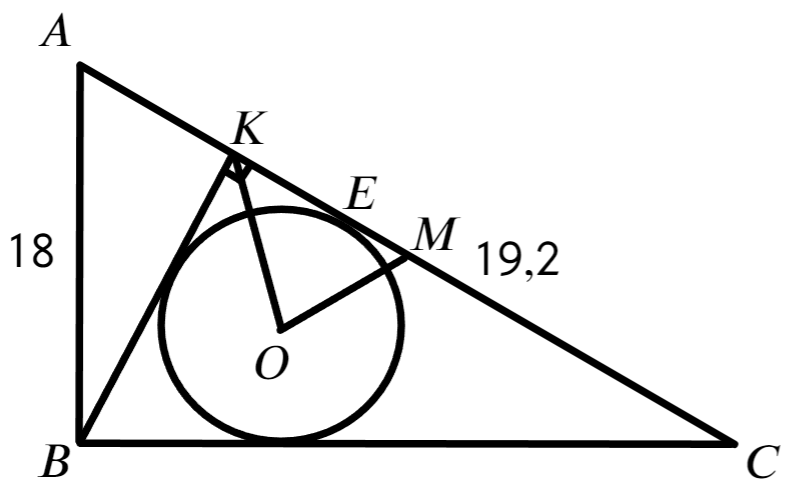
\includegraphics[scale=0.35]{g9-189.png}}
\end{figure}\\
Пусть $AK=x,$ тогда по теореме Пифагора $BK^2=324-x^2,\ BC^2=324-x^2+19,2^2,\ 324+324-x^2+19,2^2=(x+19,2)^2,$ откуда $648-x^2+19,2^2=x^2+38,4x+19,2^2,\
2x^2+38,4x-648=0,\ (x+30)(x-10,8)=0,\ x=10,8.$ Тогда $AC=10,8+19,2=30,\ BK=\sqrt{324-10,8^2}=14,4,\ BC=\sqrt{324-10,8^2+19,2^2}=24.$ Центр описанной вокруг прямоугольного треугольника окружности --- это середина гипотенузы, обозначим её буквой $M.$ Тогда $AM=30:2=15$ и $KM=15-10,8=4,2.$ Найдём радиус окружности, вписанной в треугольник $BKC:\ S=\cfrac{1}{2}\cdot14,4\cdot19,2=r\cdot\cfrac{14,4+19,2+24}{2},\ r=4,8.$ Если $E$ --- точка касания окружности со стороной $KC,$ то $KE=\cfrac{14,4+19,2-24}{2}=4,8$ и $KO=\sqrt{4,8^2+4,8^2}=4,8\sqrt{2}.$ Так как $KO$ является биссектрисой, $\angle MKO=90^\circ:2=45^\circ.$ Тогда по теореме косинусов $OM^2=46,08+17,64-2\cdot4,8\sqrt{2}\cdot4,2\cdot\cfrac{\sqrt{2}}{2}=23,4,\ OM=\cfrac{3\sqrt{26}}{10}.$\\
